% Options for packages loaded elsewhere
\PassOptionsToPackage{unicode}{hyperref}
\PassOptionsToPackage{hyphens}{url}
%
\documentclass[
  ignorenonframetext,
]{beamer}
\usepackage{pgfpages}
\setbeamertemplate{caption}[numbered]
\setbeamertemplate{caption label separator}{: }
\setbeamercolor{caption name}{fg=normal text.fg}
\beamertemplatenavigationsymbolsempty
% Prevent slide breaks in the middle of a paragraph
\widowpenalties 1 10000
\raggedbottom
\setbeamertemplate{part page}{
  \centering
  \begin{beamercolorbox}[sep=16pt,center]{part title}
    \usebeamerfont{part title}\insertpart\par
  \end{beamercolorbox}
}
\setbeamertemplate{section page}{
  \centering
  \begin{beamercolorbox}[sep=12pt,center]{part title}
    \usebeamerfont{section title}\insertsection\par
  \end{beamercolorbox}
}
\setbeamertemplate{subsection page}{
  \centering
  \begin{beamercolorbox}[sep=8pt,center]{part title}
    \usebeamerfont{subsection title}\insertsubsection\par
  \end{beamercolorbox}
}
\AtBeginPart{
  \frame{\partpage}
}
\AtBeginSection{
  \ifbibliography
  \else
    \frame{\sectionpage}
  \fi
}
\AtBeginSubsection{
  \frame{\subsectionpage}
}
\usepackage{amsmath,amssymb}
\usepackage{iftex}
\ifPDFTeX
  \usepackage[T1]{fontenc}
  \usepackage[utf8]{inputenc}
  \usepackage{textcomp} % provide euro and other symbols
\else % if luatex or xetex
  \usepackage{unicode-math} % this also loads fontspec
  \defaultfontfeatures{Scale=MatchLowercase}
  \defaultfontfeatures[\rmfamily]{Ligatures=TeX,Scale=1}
\fi
\usepackage{lmodern}
\usetheme[]{Madrid}
\usefonttheme{structurebold}
\ifPDFTeX\else
  % xetex/luatex font selection
\fi
% Use upquote if available, for straight quotes in verbatim environments
\IfFileExists{upquote.sty}{\usepackage{upquote}}{}
\IfFileExists{microtype.sty}{% use microtype if available
  \usepackage[]{microtype}
  \UseMicrotypeSet[protrusion]{basicmath} % disable protrusion for tt fonts
}{}
\makeatletter
\@ifundefined{KOMAClassName}{% if non-KOMA class
  \IfFileExists{parskip.sty}{%
    \usepackage{parskip}
  }{% else
    \setlength{\parindent}{0pt}
    \setlength{\parskip}{6pt plus 2pt minus 1pt}}
}{% if KOMA class
  \KOMAoptions{parskip=half}}
\makeatother
\usepackage{xcolor}
\newif\ifbibliography
\usepackage{graphicx}
\makeatletter
\def\maxwidth{\ifdim\Gin@nat@width>\linewidth\linewidth\else\Gin@nat@width\fi}
\def\maxheight{\ifdim\Gin@nat@height>\textheight\textheight\else\Gin@nat@height\fi}
\makeatother
% Scale images if necessary, so that they will not overflow the page
% margins by default, and it is still possible to overwrite the defaults
% using explicit options in \includegraphics[width, height, ...]{}
\setkeys{Gin}{width=\maxwidth,height=\maxheight,keepaspectratio}
% Set default figure placement to htbp
\makeatletter
\def\fps@figure{htbp}
\makeatother
\setlength{\emergencystretch}{3em} % prevent overfull lines
\providecommand{\tightlist}{%
  \setlength{\itemsep}{0pt}\setlength{\parskip}{0pt}}
\setcounter{secnumdepth}{-\maxdimen} % remove section numbering
\ifLuaTeX
  \usepackage{selnolig}  % disable illegal ligatures
\fi
\usepackage{bookmark}
\IfFileExists{xurl.sty}{\usepackage{xurl}}{} % add URL line breaks if available
\urlstyle{same}
\hypersetup{
  pdftitle={Optimisation du placement des antennes au Sénégal: cas Kédougou, Tambacounda et Matam},
  pdfauthor={SOMA Ben Idriss Diloma},
  hidelinks,
  pdfcreator={LaTeX via pandoc}}

\title{Optimisation du placement des antennes au Sénégal: cas Kédougou,
Tambacounda et Matam}
\author{SOMA Ben Idriss Diloma}
\date{2025-07-07}

\begin{document}
\frame{\titlepage}

\begin{frame}[allowframebreaks]
  \tableofcontents[hideallsubsections]
\end{frame}
\section{Introduction}\label{introduction}

\begin{frame}{Introduction}
\begin{itemize}
\tightlist
\item
  La connectivité mobile reste inégale au Sénégal, surtout dans les
  zones rurales.
\item
  Le placement des antennes est un levier stratégique pour :

  \begin{itemize}
  \tightlist
  \item
    améliorer la \textbf{couverture réseau},
  \item
    \textbf{réduire les interférences},
  \item
    et \textbf{optimiser les coûts}.
  \end{itemize}
\item
  Le projet s'appuie sur un \textbf{modèle de simulation} tenant compte
  :

  \begin{itemize}
  \tightlist
  \item
    de la \textbf{propagation des ondes},
  \item
    des \textbf{contraintes géographiques et budgétaires},
  \item
    et de l'\textbf{allocation des fréquences}.
  \end{itemize}
\end{itemize}
\end{frame}

\begin{frame}{Contexte général}
\phantomsection\label{contexte-guxe9nuxe9ral}
\textbf{Problématique :} Le placement des antennes de télécommunication
est crucial pour assurer une couverture réseau optimale, surtout dans
les régions rurales du Sénégal.

\textbf{Défis de la connectivité au Sénégal :}

\begin{itemize}
\tightlist
\item
  Couverture inégale entre zones urbaines et rurales
\item
  Qualité de service limitée dans les zones reculées
\item
  Fracture numérique impactant le développement
\item
  Contraintes géographiques et économiques
\end{itemize}

\textbf{Enjeux du placement des antennes :}

\begin{itemize}
\tightlist
\item
  Assurer une couverture efficace
\item
  Minimiser les interférences
\item
  Optimiser les coûts d'installation
\item
  Respecter les contraintes techniques
\end{itemize}
\end{frame}

\begin{frame}{Objectifs du projet}
\phantomsection\label{objectifs-du-projet}
\textbf{Objectif principal :} Optimiser le placement des antennes pour
une meilleure couverture réseau tout en réduisant les interférences
\end{frame}

\section{Zone d'étude}\label{zone-duxe9tude}

\begin{frame}{Zone d'étude}
Nous nous concentrons sur trois régions du Sénégal : Kédougou,
Tambacounda et Matam. Ces régions présentent des défis uniques en
matière de connectivité mobile, notamment en raison de leur géographie
et de leur densité de population. Ces régions présente,nt des taux de
couverture réseau de .
\end{frame}

\section{Vue d'ensemble du Sénégal de la couverture
reseau}\label{vue-densemble-du-suxe9nuxe9gal-de-la-couverture-reseau}

\begin{frame}{Carte de la couverture réseau}
\phantomsection\label{carte-de-la-couverture-ruxe9seau}
\begin{center}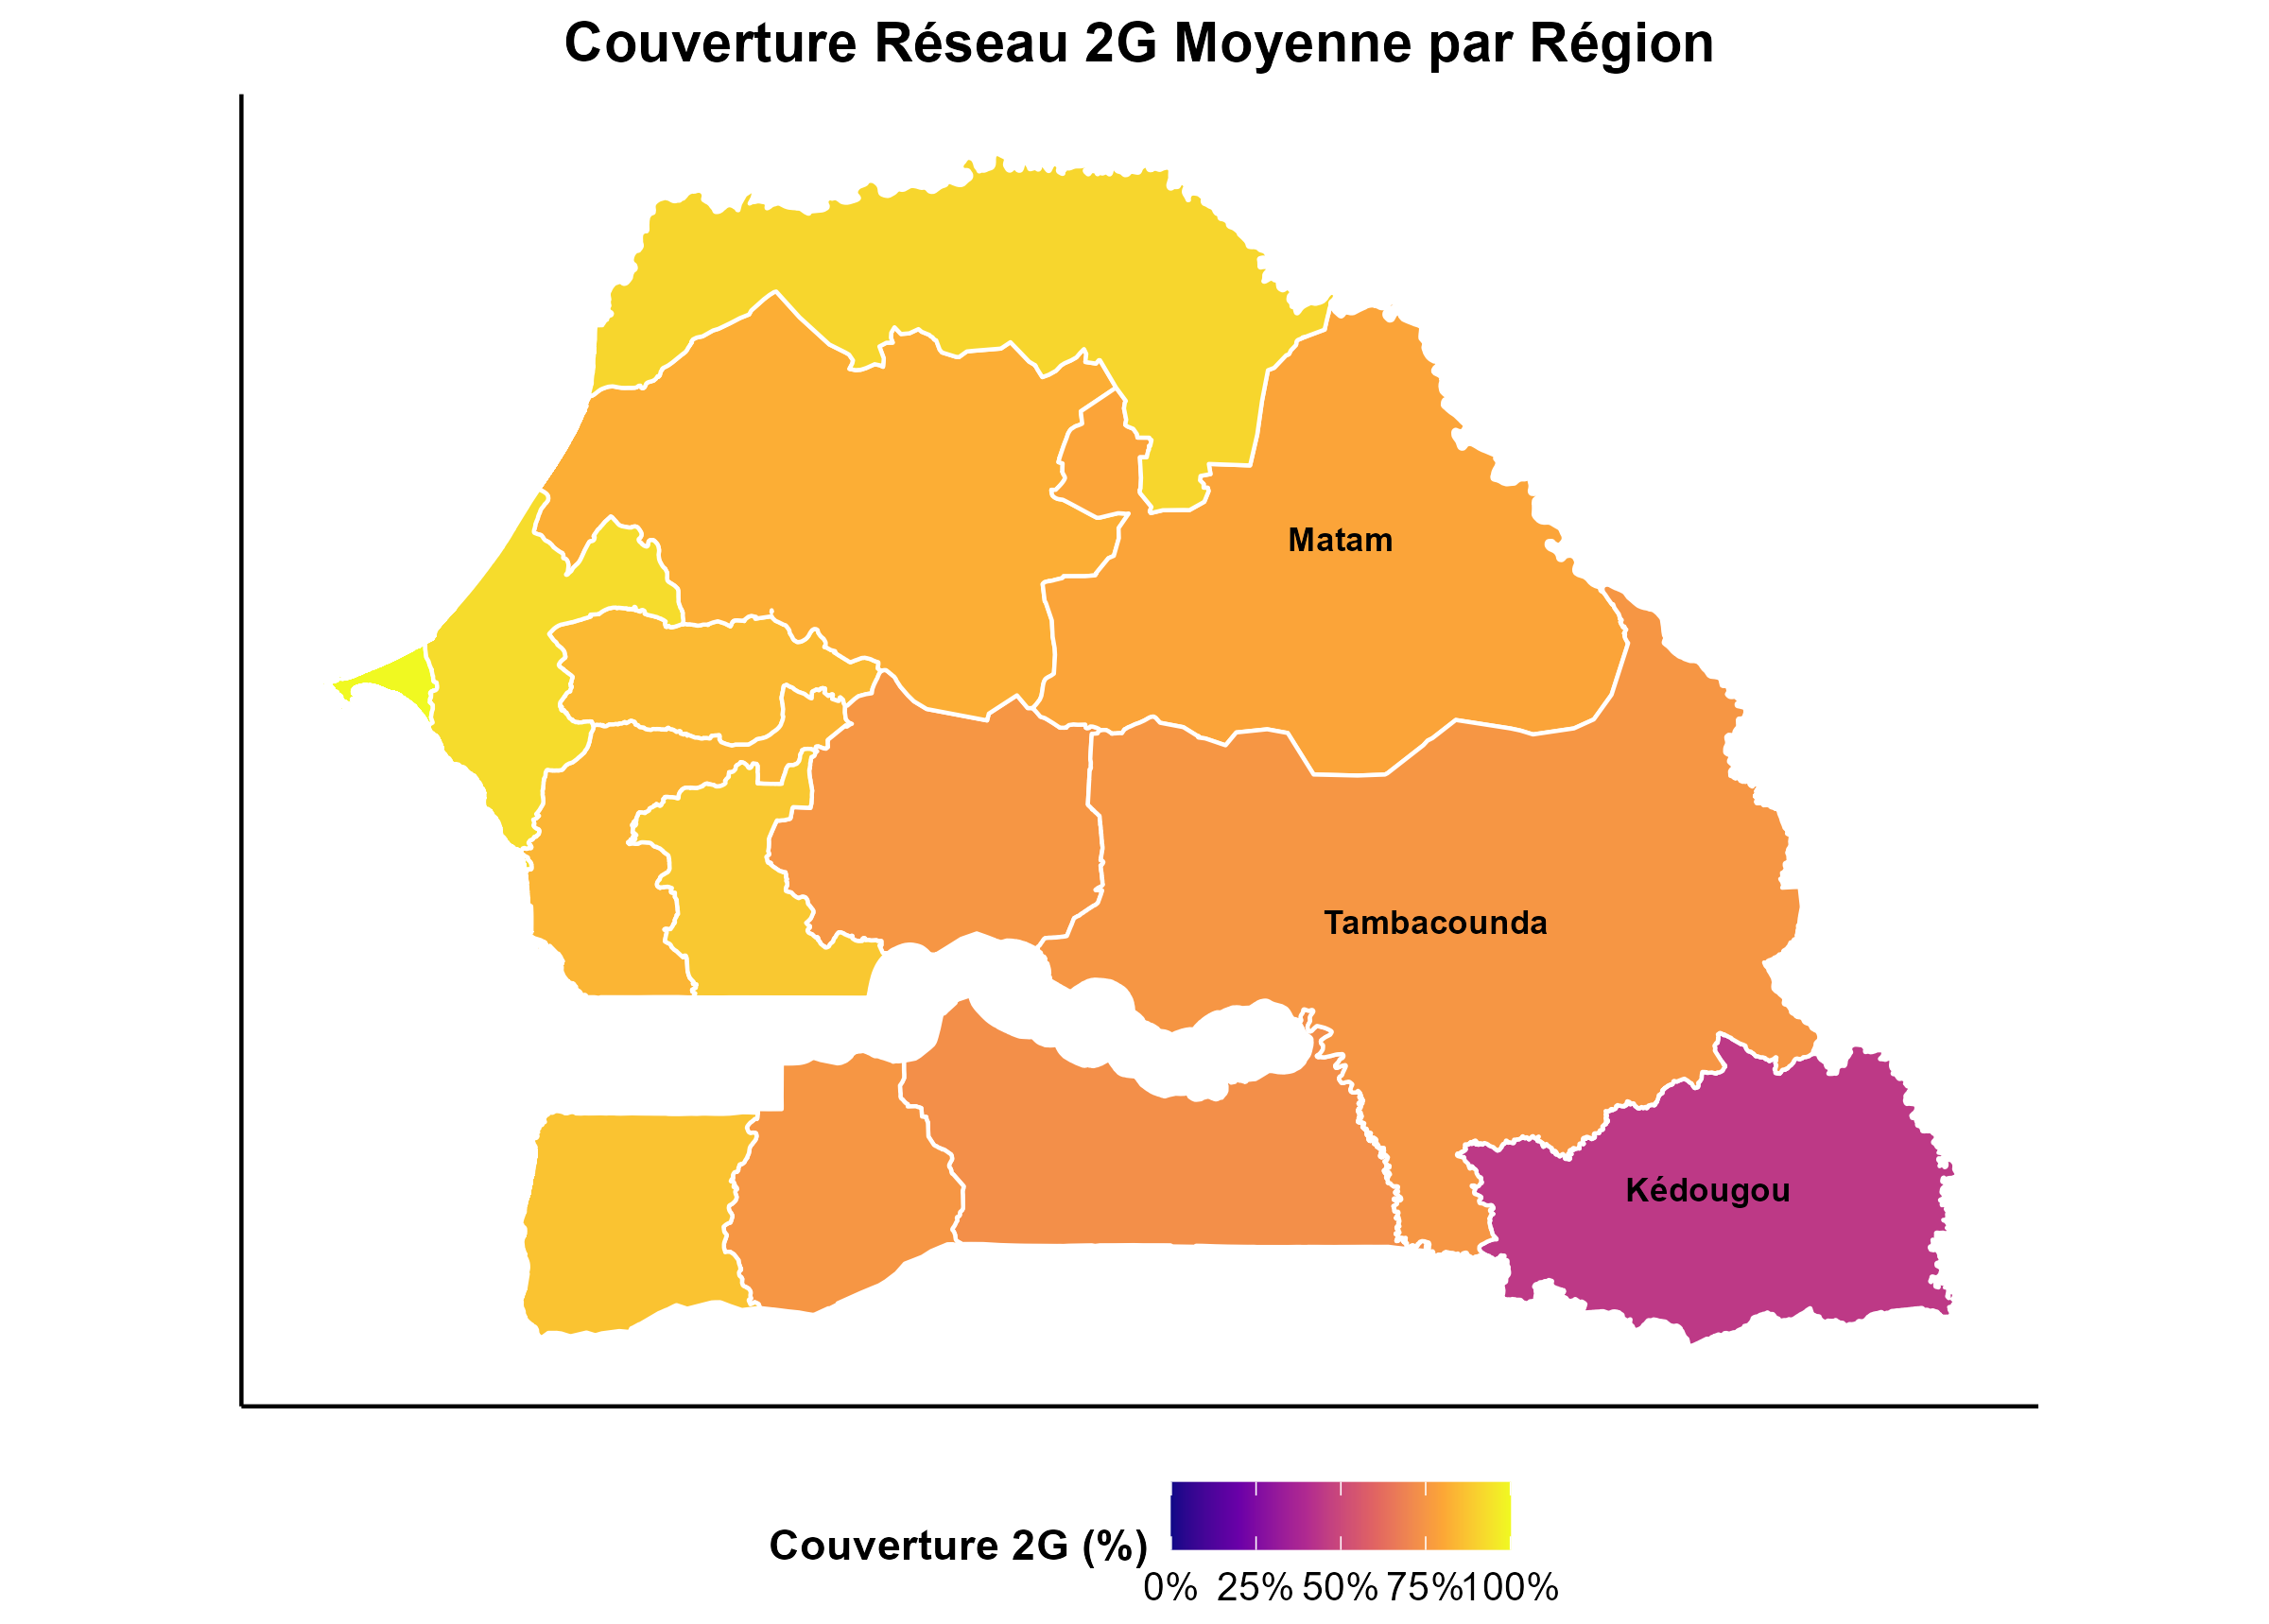
\includegraphics[width=1\linewidth]{images/carte_couverture_2G} \end{center}
\end{frame}

\begin{frame}
\begin{center}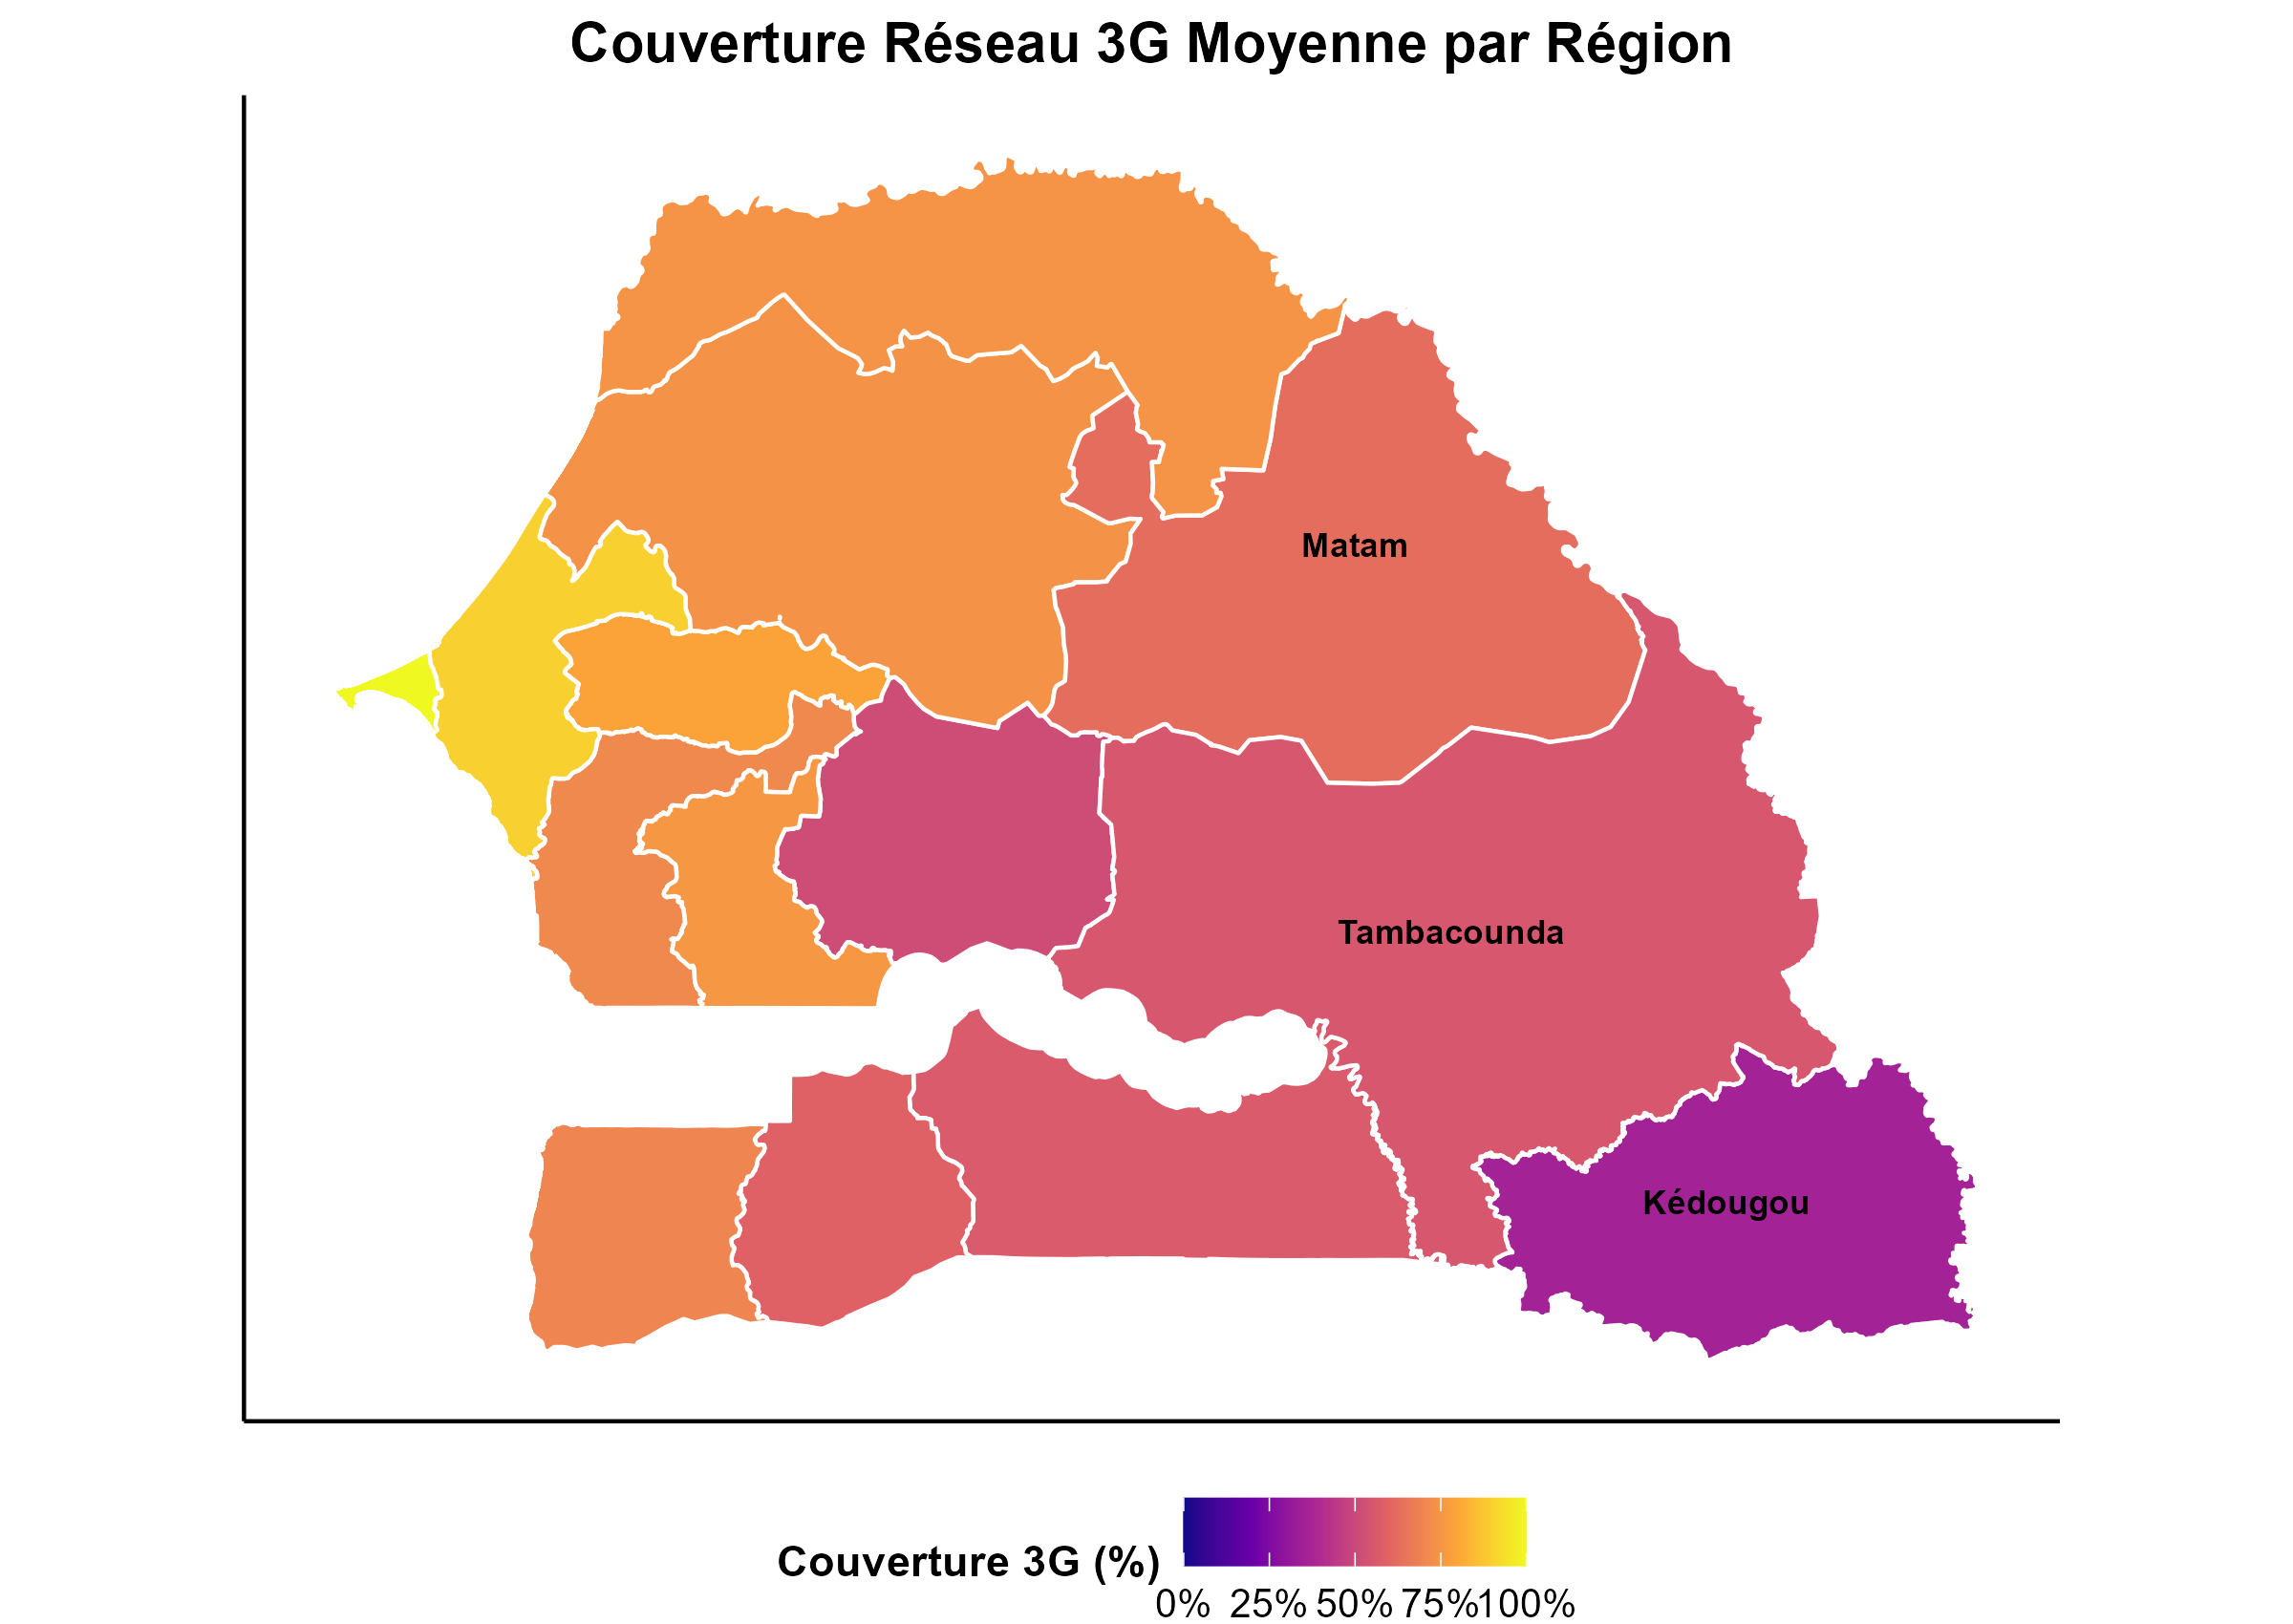
\includegraphics[width=1\linewidth]{images/carte_couverture_3G} \end{center}
\end{frame}

\begin{frame}
\begin{center}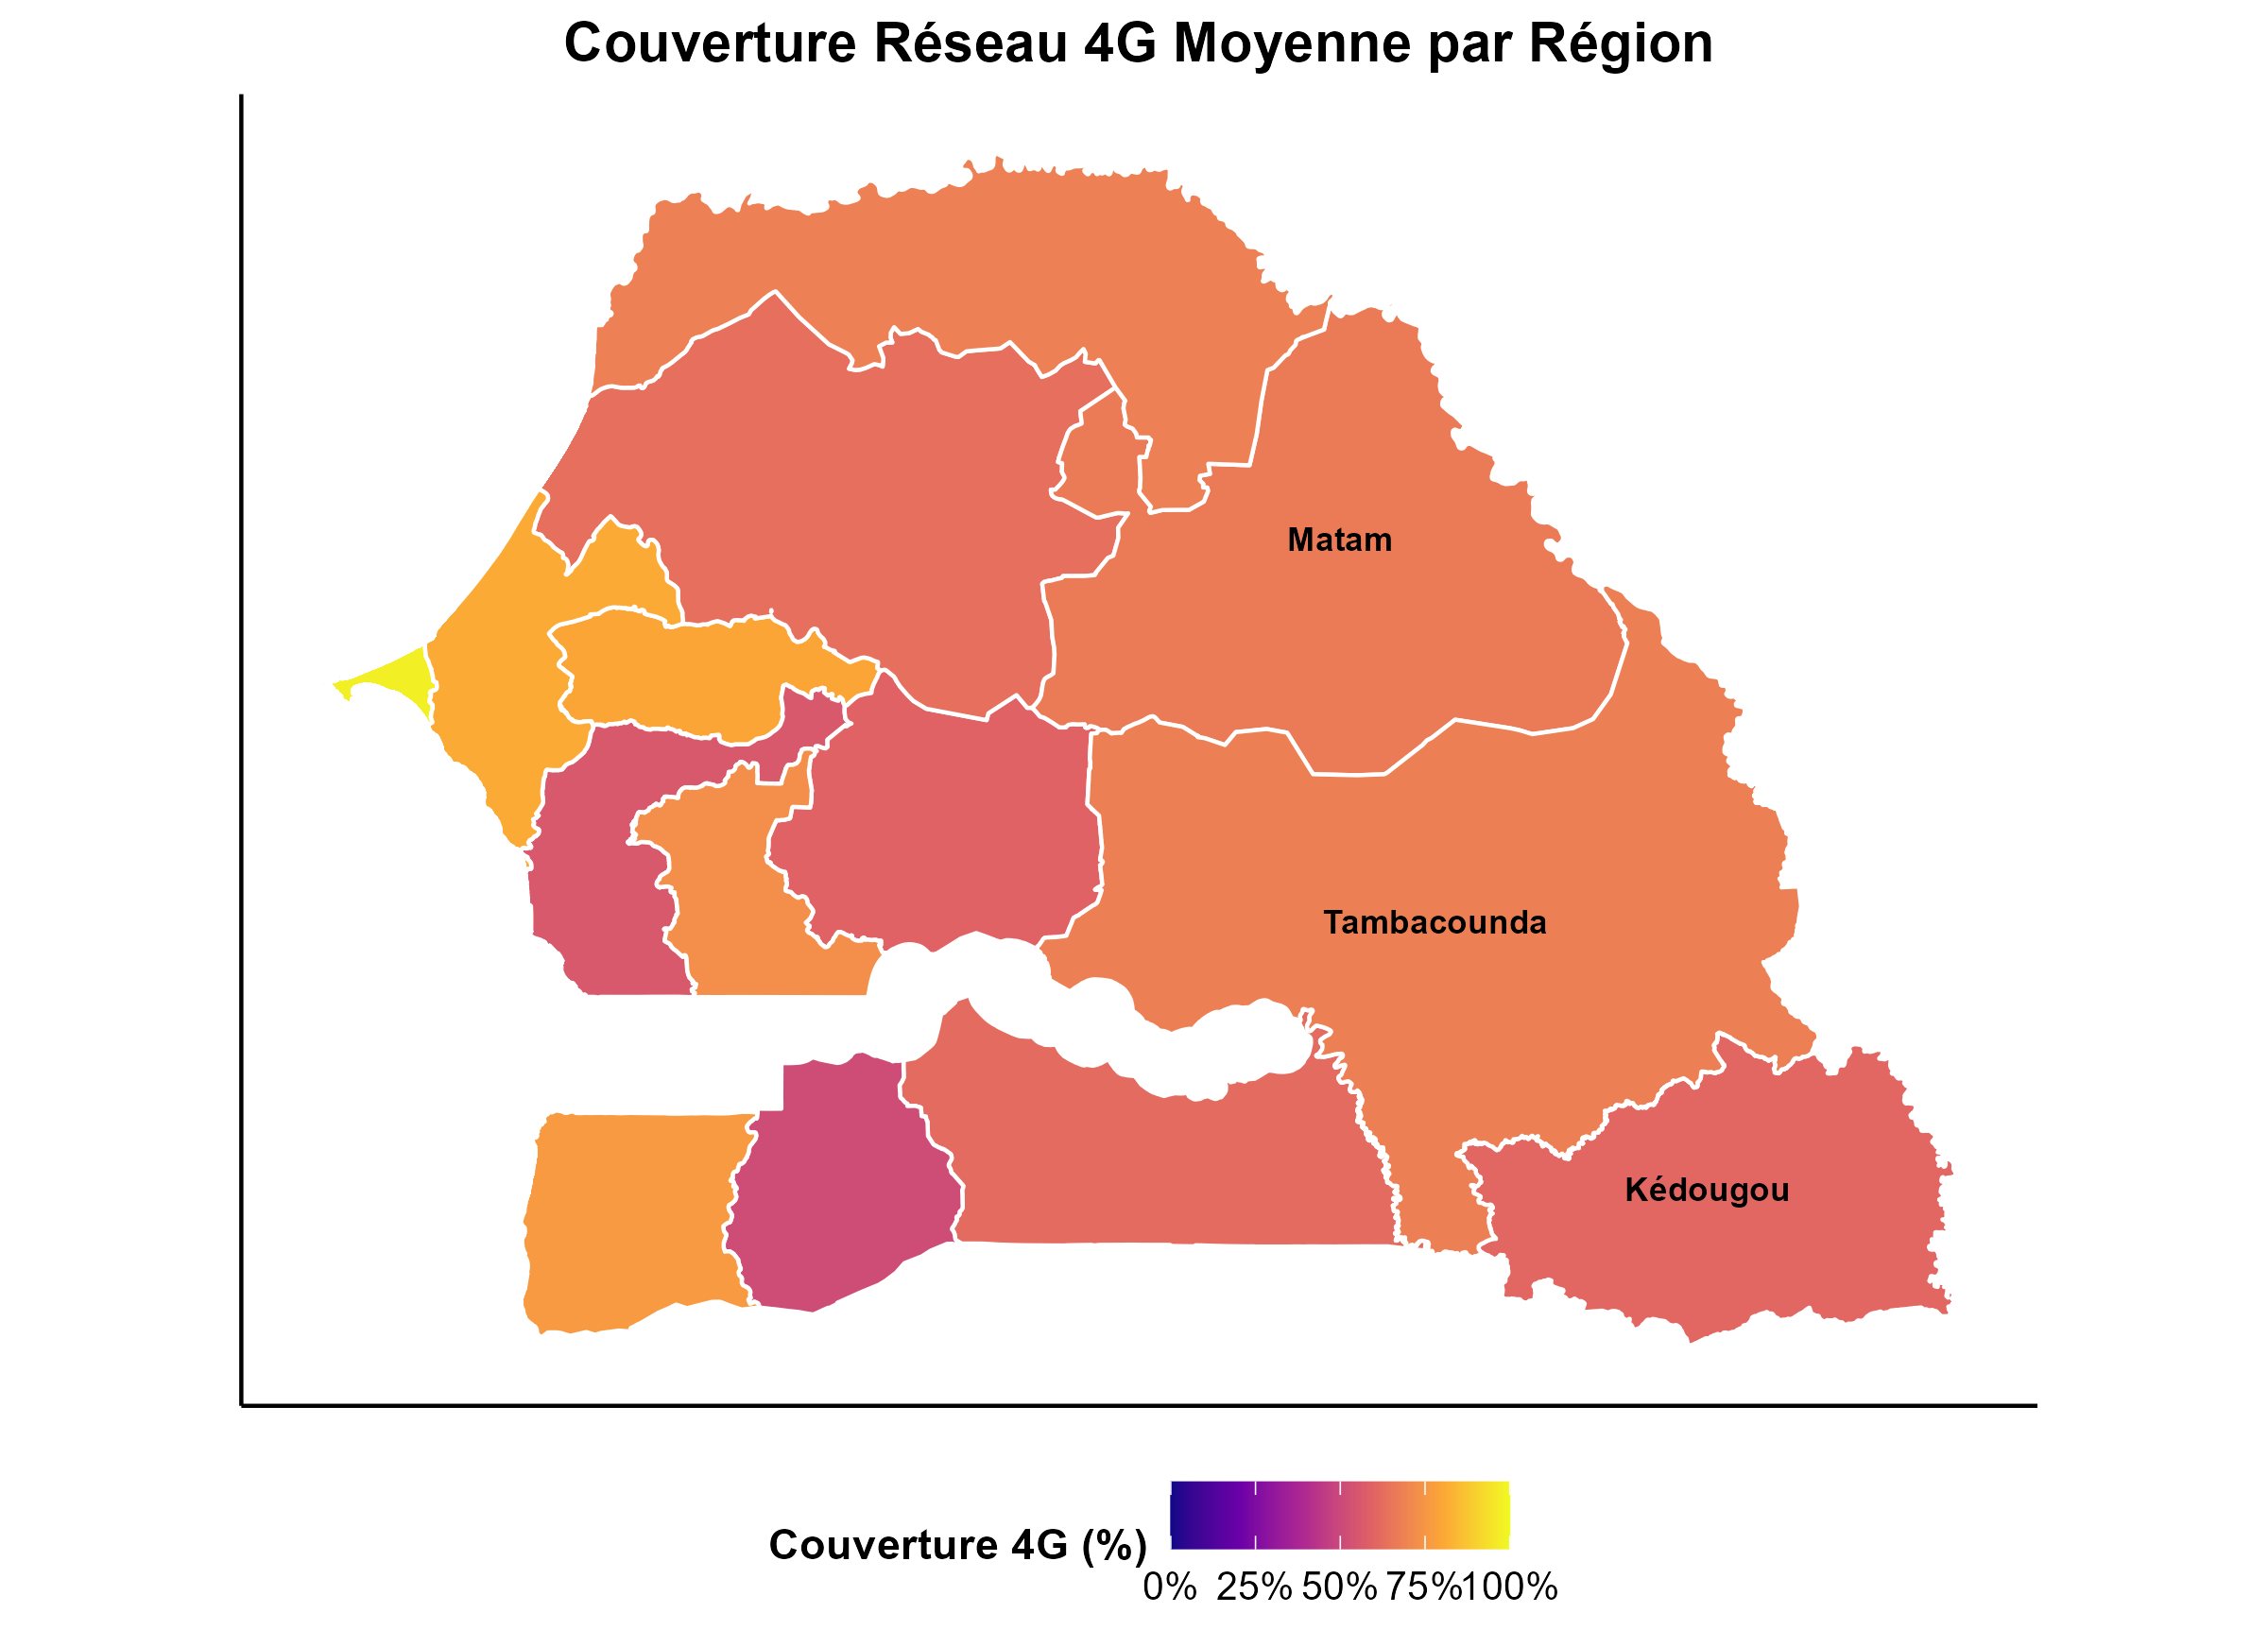
\includegraphics[width=1\linewidth]{images/carte_couverture_4G} \end{center}
\end{frame}

\begin{frame}
La carte de couverture 4G montre une concentration de la couverture dans
les grandes villes notamment à Dakar , tandis que les zones rurales
restent largement sous-couvertes, avec des débits souvent insuffisants
pour les usages modernes.

\begin{center}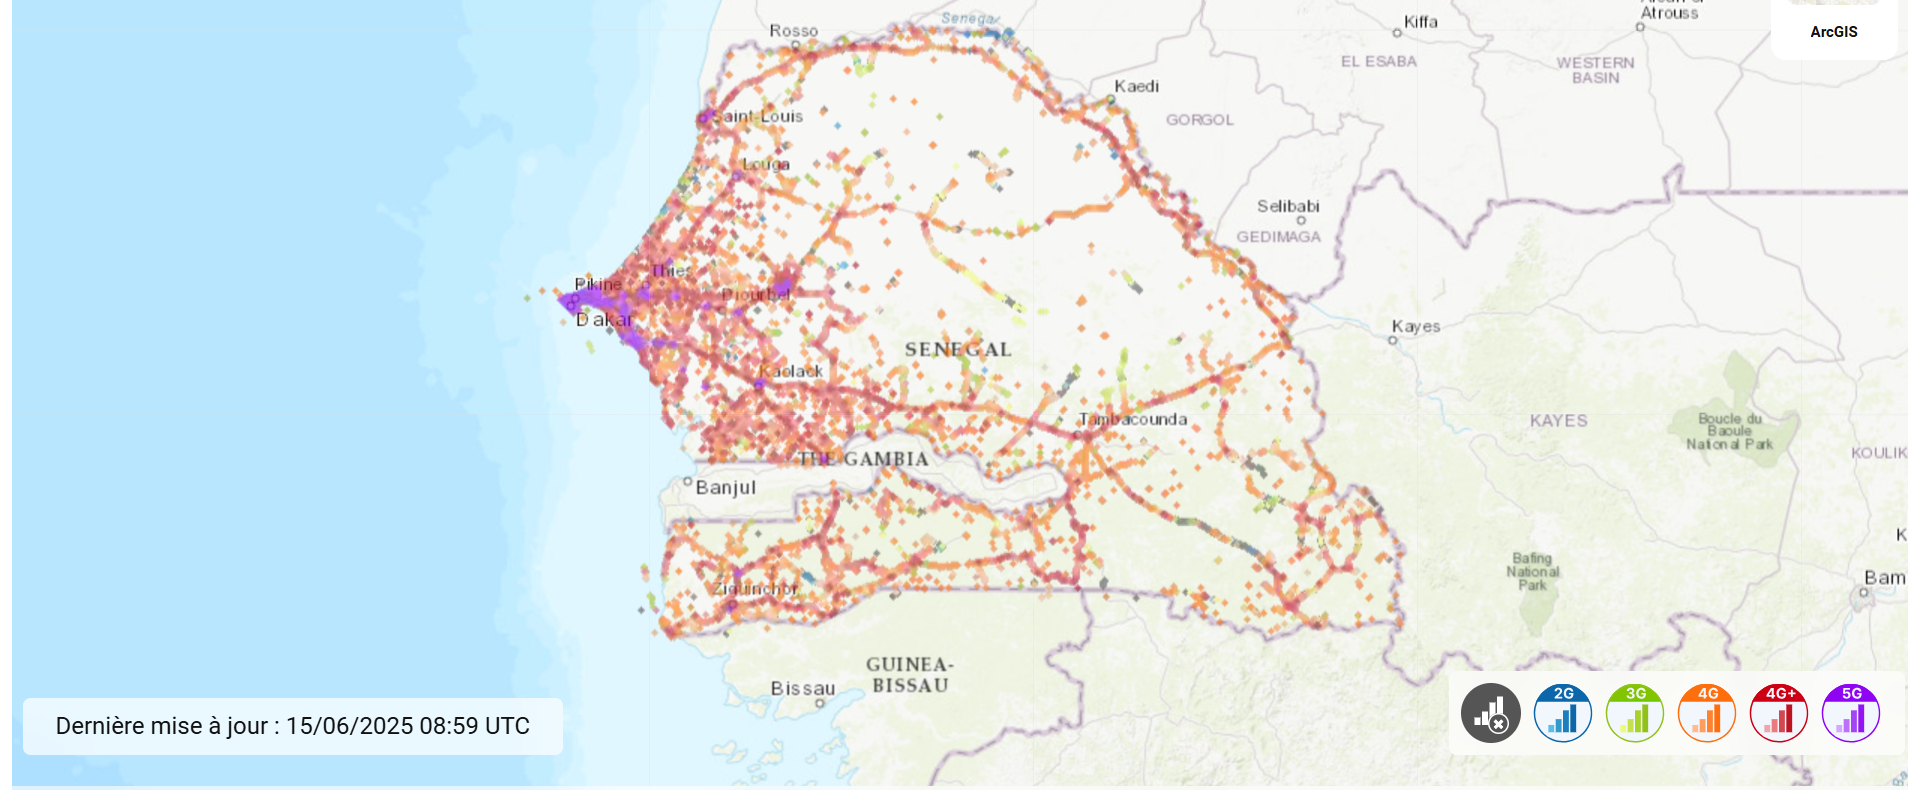
\includegraphics[width=1\linewidth]{images/nperfcouverture_orange} \end{center}

le réseau Orange est le plus étendu, avec une couverture de 95\% dans la
région de Dakar, mais il reste des zones blanches dans les régions
rurales. le réseau 4G de Free est beaucoup plus concentré dans les zones
urbaines, , mais il est très limité dans les zones rurales.

\begin{center}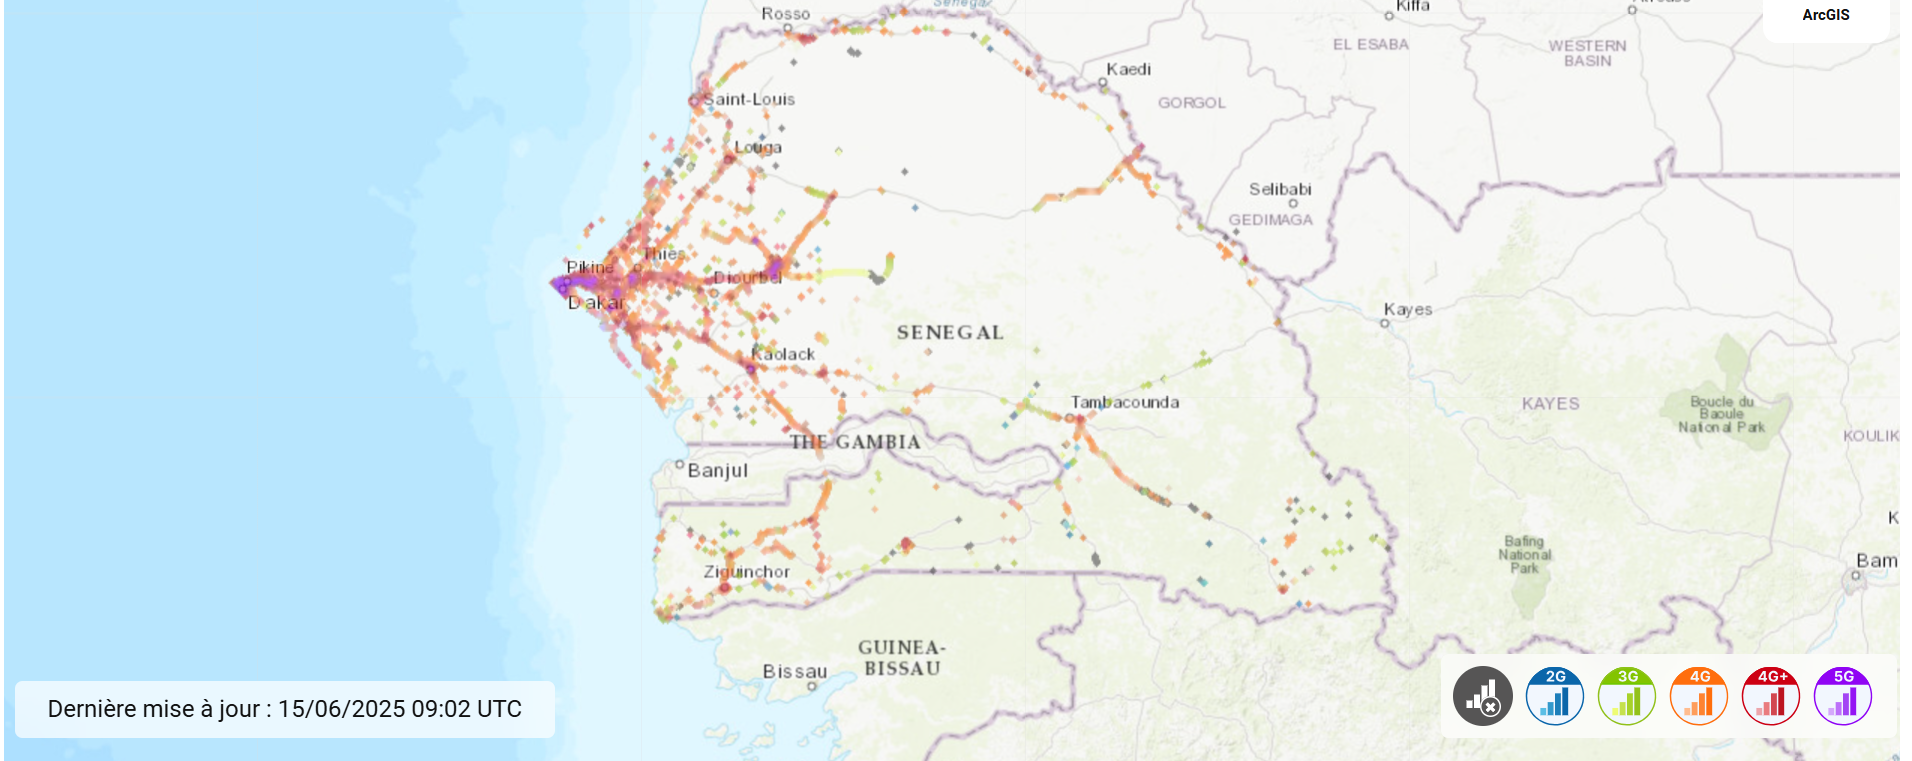
\includegraphics[width=1\linewidth]{images/nperfcouverture_free} \end{center}

la couverture de Free est légèrement inférieure, avec 90\% dans la
région de Dakar, mais elle souffre également de lacunes dans les zones
rurales.

\begin{center}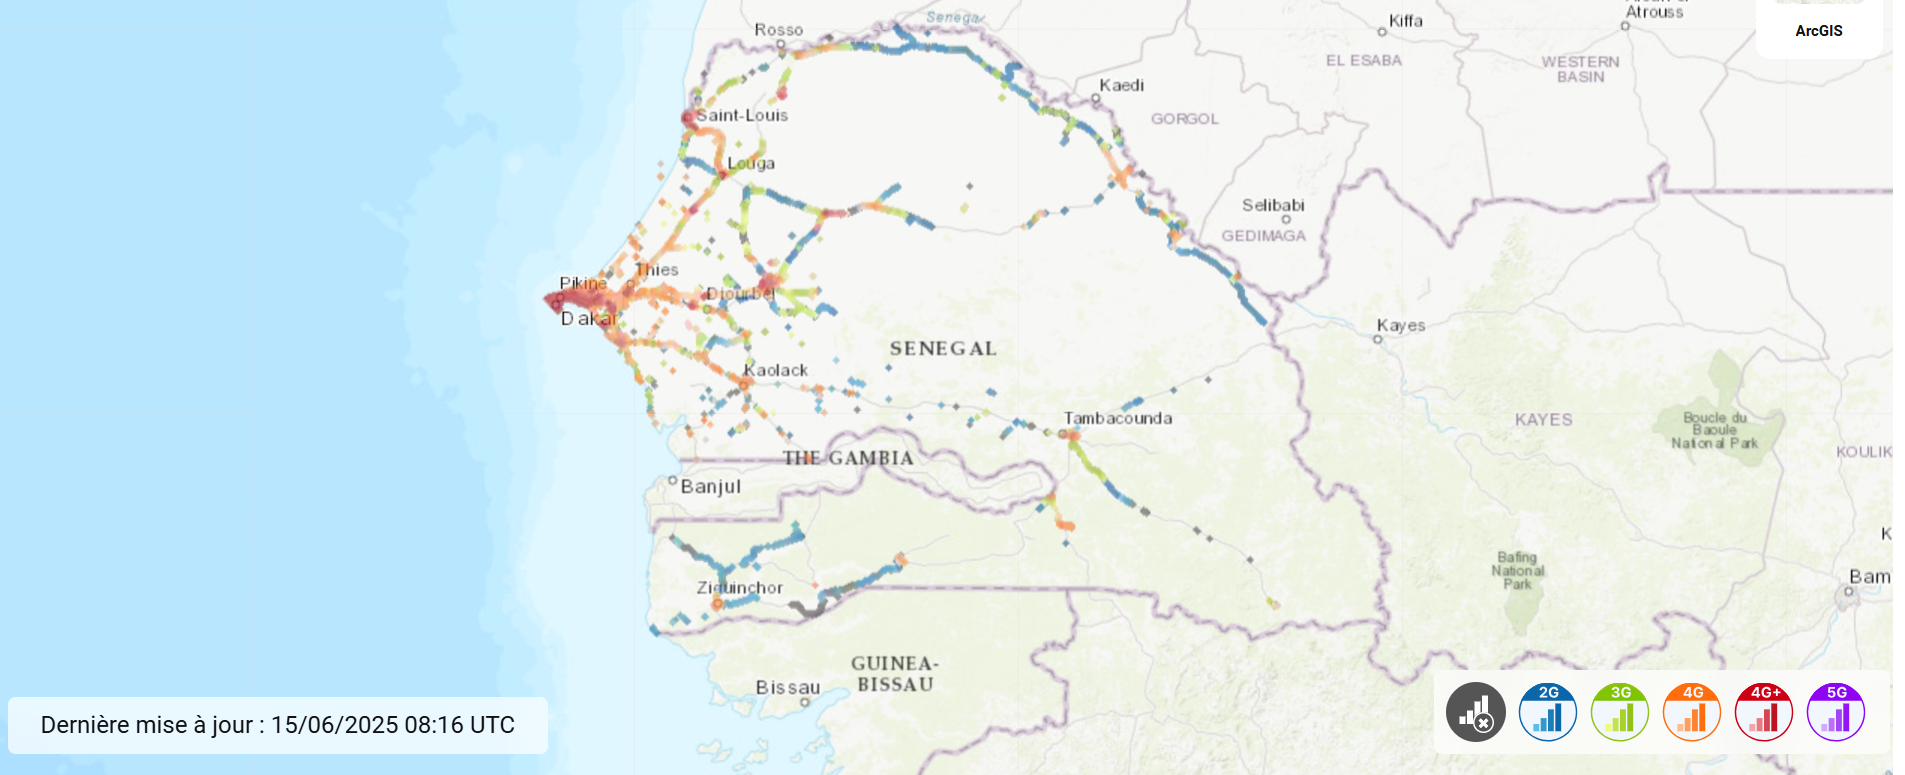
\includegraphics[width=1\linewidth]{images/nperfcouverture_express} \end{center}
\end{frame}

\begin{frame}{Présentation des régions cibles}
\phantomsection\label{pruxe9sentation-des-ruxe9gions-cibles}
\textbf{Régions étudiées :} Kédougou, Tambacounda et Matam

\textbf{Caractéristiques communes :}

\begin{itemize}
\tightlist
\item
  Situées dans la partie orientale du Sénégal
\item
  Diversité géographique et culturelle
\item
  Faible taux de couverture réseau
\item
  Disparités importantes urbain/rural
\end{itemize}

\textbf{Défis spécifiques :}

\begin{itemize}
\tightlist
\item
  Manque d'infrastructures de télécommunication
\item
  Accès limité à Internet et services mobiles
\item
  Population principalement rurale
\item
  Contraintes géographiques importantes
\end{itemize}
\end{frame}

\begin{frame}{Indicateurs clés du Sénégal}
\phantomsection\label{indicateurs-cluxe9s-du-suxe9nuxe9gal}
\textbf{Données démographiques et géographiques :}

\begin{itemize}
\tightlist
\item
  Population : \textgreater{} 18 millions d'habitants (2023)
\item
  Superficie : 196 722 km²
\item
  Taux d'urbanisation : \textasciitilde47\%
\item
  Accès à Internet : \textasciitilde58\% (2022)
\end{itemize}

\textbf{Répartition administrative :}

\begin{itemize}
\tightlist
\item
  14 régions administratives
\item
  Concentration des infrastructures dans l'ouest
\item
  Zones rurales sous-connectées
\end{itemize}
\end{frame}

\section{État de la couverture
réseau}\label{uxe9tat-de-la-couverture-ruxe9seau}

\begin{frame}{Couverture par opérateur}
\phantomsection\label{couverture-par-opuxe9rateur}
\begin{figure}
\centering
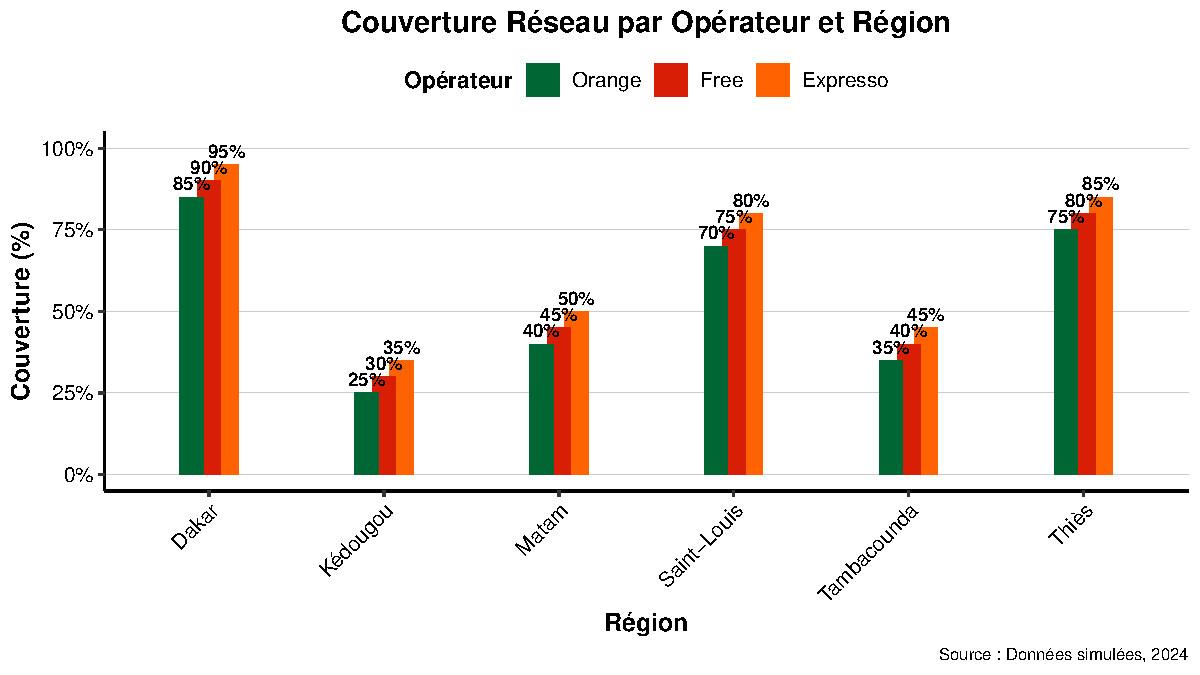
\includegraphics{beamer_files/figure-beamer/operator-coverage-1.pdf}
\caption{Comparaison de la couverture réseau par opérateur}
\end{figure}
\end{frame}

\begin{frame}{Analyse de la couverture}
\phantomsection\label{analyse-de-la-couverture}
\textbf{Constats principaux :}

\begin{itemize}
\tightlist
\item
  Orange : réseau le plus étendu (95\% à Dakar, mais zones blanches
  rurales)
\item
  Free : couverture concentrée en zones urbaines (90\% à Dakar)
\item
  Expresso : couverture la plus faible (85\% à Dakar, \textless50\%
  zones rurales)
\end{itemize}

\textbf{Disparités régionales :}

\begin{itemize}
\tightlist
\item
  Kédougou et Tambacounda : couverture \textless50\% tous opérateurs
\item
  Matam : couverture variable selon l'opérateur
\item
  Concentration des infrastructures dans l'ouest du pays
\end{itemize}
\end{frame}

\section{Généralités sur les réseaux de
télécommunication}\label{guxe9nuxe9ralituxe9s-sur-les-ruxe9seaux-de-tuxe9luxe9communication}

\begin{frame}{Canaux de communication}
\phantomsection\label{canaux-de-communication}
\textbf{Définition :} Médium de transmission d'information permettant
l'acheminement d'un message

\textbf{Types de supports :}

\begin{itemize}
\tightlist
\item
  Support physique (câble)
\item
  Support logique (canal radio)
\end{itemize}

\textbf{Caractéristiques importantes :}

\begin{itemize}
\tightlist
\item
  Bande passante du canal
\item
  Capacité de transmission
\item
  Susceptibilité aux interférences
\end{itemize}
\end{frame}

\begin{frame}{Spectre de fréquence et modulation}
\phantomsection\label{spectre-de-fruxe9quence-et-modulation}
\begin{figure}
\centering
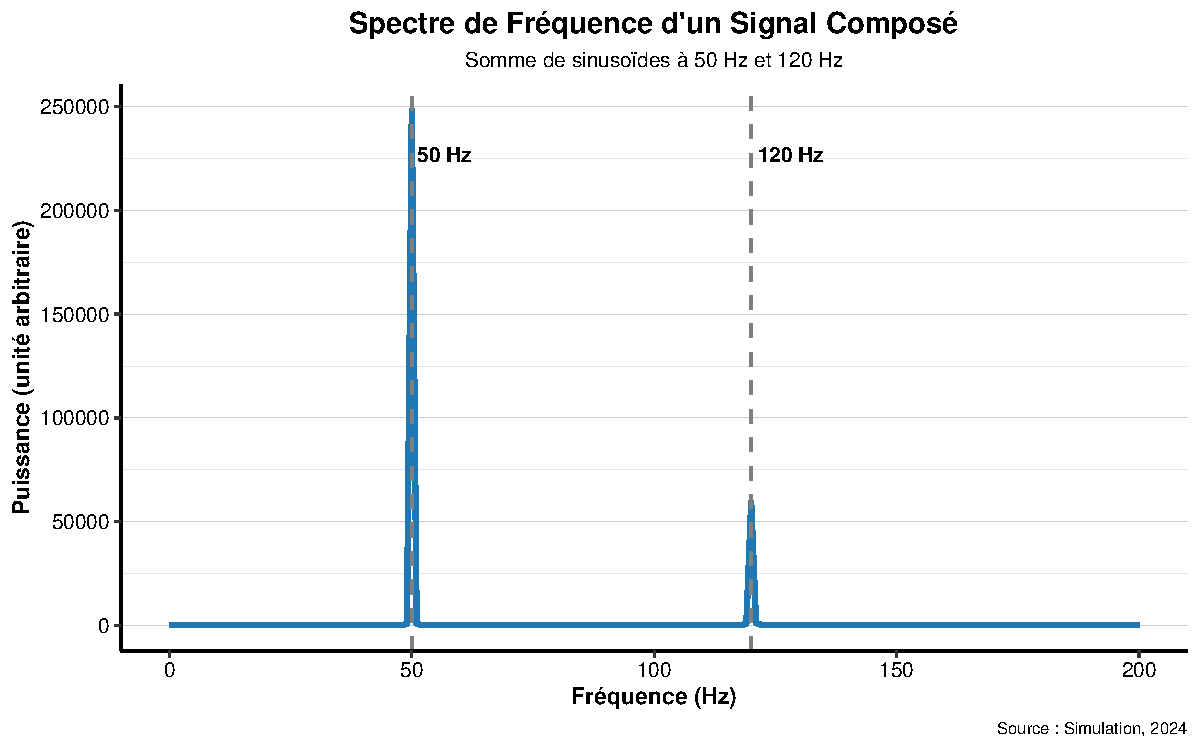
\includegraphics{beamer_files/figure-beamer/frequency-spectrum-1.pdf}
\caption{Spectre de fréquence d'un signal composé}
\end{figure}
\end{frame}

\begin{frame}{Modulation du signal}
\phantomsection\label{modulation-du-signal}
\begin{figure}
\centering
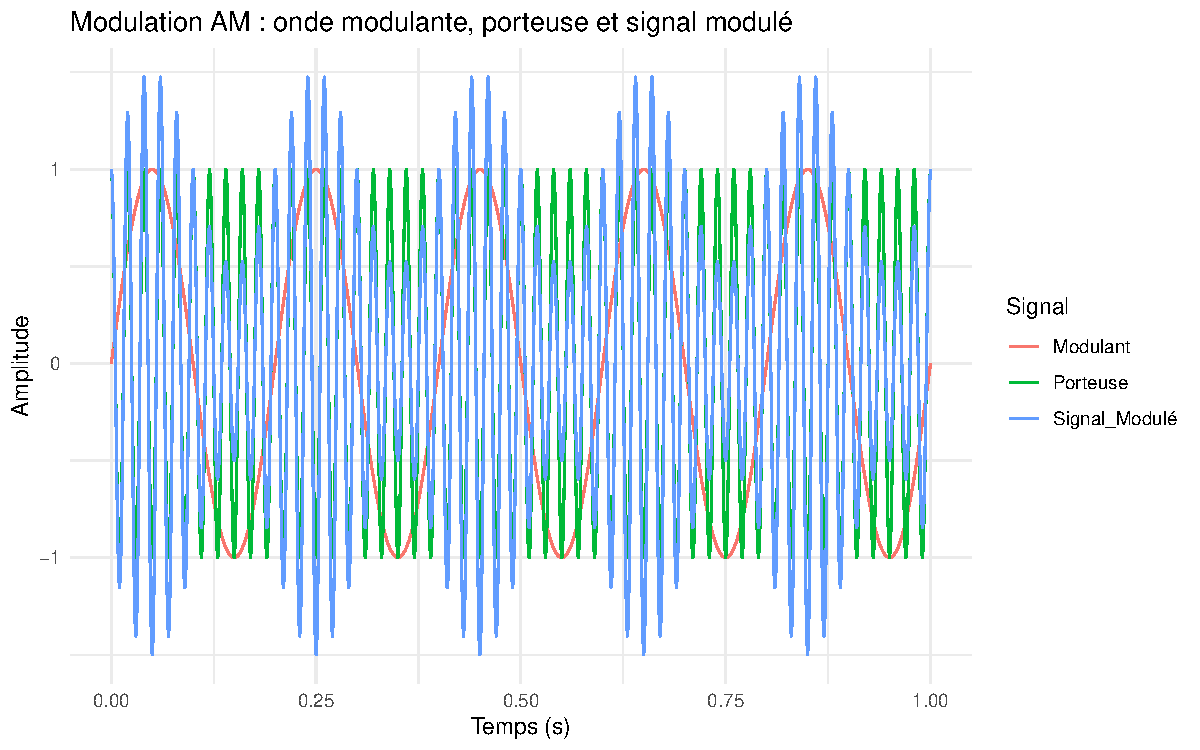
\includegraphics{beamer_files/figure-beamer/modulation-1.pdf}
\caption{Modulation d'amplitude : modulant, porteuse et signal modulé}
\end{figure}
\end{frame}

\begin{frame}{Capacité d'un canal - Théorie de Shannon}
\phantomsection\label{capacituxe9-dun-canal---thuxe9orie-de-shannon}
\textbf{Formule de Shannon :}

\[C_I = \Delta f \cdot \log_2 \left(1 + \frac{P_S}{P_N} \right)\]

\textbf{Où :}

\begin{itemize}
\tightlist
\item
  \(C_I\) : capacité du canal (bits/s)
\item
  \(\Delta f\) : largeur de bande (Hz)
\item
  \(P_S\) : puissance du signal reçu
\item
  \(P_N\) : puissance du bruit
\end{itemize}

\textbf{Implications :}

\begin{itemize}
\tightlist
\item
  Plus la bande passante est large, plus la capacité est élevée
\item
  Importance du rapport signal/bruit (SNR)
\item
  Nécessité de gérer efficacement le spectre
\end{itemize}
\end{frame}

\section{Propagation des ondes}\label{propagation-des-ondes}

\begin{frame}{Modèle de Friis (espace libre)}
\phantomsection\label{moduxe8le-de-friis-espace-libre}
\textbf{Équation de Friis :}

\[P_r(d) = \frac{P_t G_t G_r \lambda^2}{(4 \pi d)^2 L}\]

\textbf{En fonction de la fréquence :}

\[P_r(d) = \frac{P_e G_e G_r c^2}{(4 \pi d f)^2}\]

\textbf{Points clés :}

\begin{itemize}
\tightlist
\item
  Atténuation proportionnelle à \(d^{-2}\)
\item
  Dépendance à \(f^{-2}\) : hautes fréquences portent moins loin
\item
  Modèle idéalisé sans obstacles
\end{itemize}
\end{frame}

\begin{frame}{Simulation du modèle de Friis}
\phantomsection\label{simulation-du-moduxe8le-de-friis}
\begin{figure}
\centering
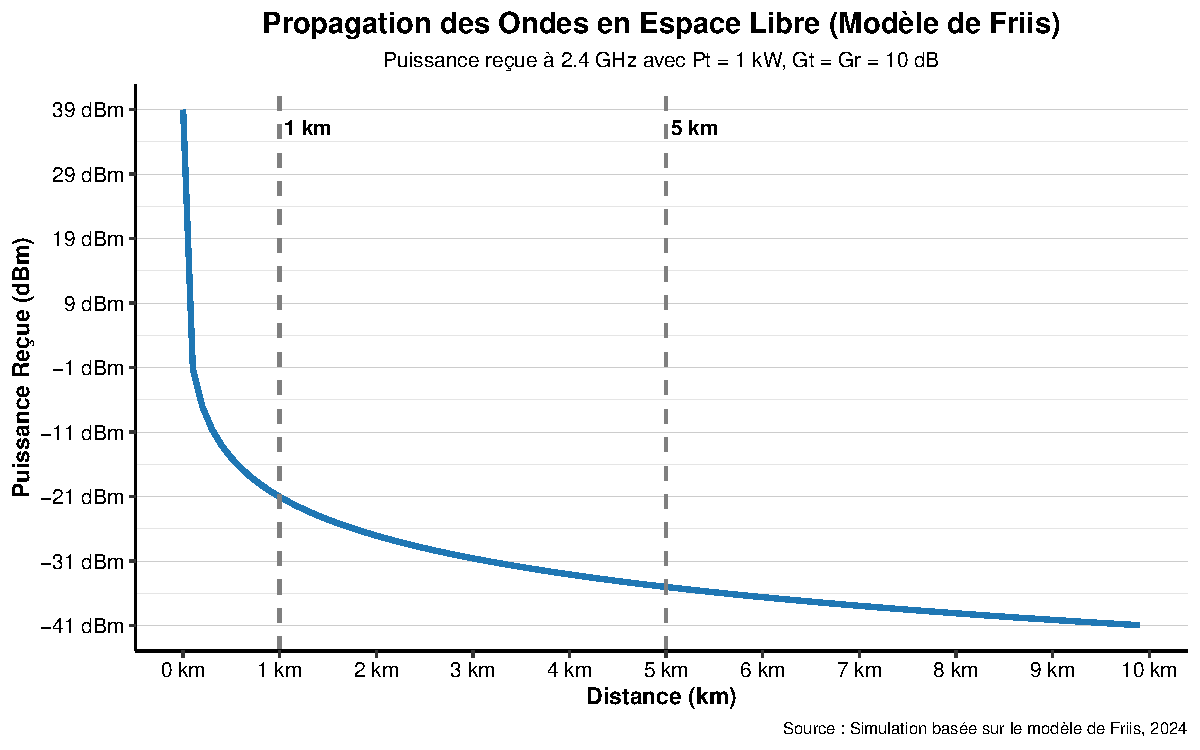
\includegraphics{beamer_files/figure-beamer/friis-model-1.pdf}
\caption{Puissance reçue en fonction de la distance (modèle de Friis)}
\end{figure}
\end{frame}

\section{Rapport signal-bruit}\label{rapport-signal-bruit}

\begin{frame}{Définition du rapport signal-bruit (SNR)}
\phantomsection\label{duxe9finition-du-rapport-signal-bruit-snr}
Le rapport signal-bruit, souvent noté SIR (pour Signal to Interference
Ratio), est défini comme le rapport entre la puissance reçue d'une
source PS et la puissance des interférences perturbant la réception PI :
\[
\text{SNR} = \frac{P_{signal}}{P_{bruit}}
\]

\textbf{Où :} - \(P_{signal}\) : puissance du signal utile -
\(P_{bruit}\) : puissance du bruit de fond

ou encore en décibels

\[
\text{SIR}_{dB} = 10 \log_{10} \left( \frac{P_{signal}}{P_{bruit}} \right)
\]
\end{frame}

\begin{frame}{Zone de couverture}
\phantomsection\label{zone-de-couverture}
La \textbf{zone de couverture} d'une antenne est définie comme
l'ensemble des points où la puissance reçue dépasse un seuil minimal,
généralement fixé par l'opérateur.La zone de couverture d'une antenne
est l'ensemble des points du plan où la qualité du signal reçu de cette
antenne est suffisante pour pouvoir effectuer une communica tion. Elle
est définie à partir du rapport signal-bruit, de la façon suivante : \[
\text{Zone de couverture} = \{ x \in \mathbb{R}^2 \mid \text{SIR}(x) \geq \theta \}
\]
\end{frame}

\begin{frame}{Propagation en présence d'obstacles}
\phantomsection\label{propagation-en-pruxe9sence-dobstacles}
En présence d'obstacles, la propagation des ondes est modifiée par des
phénomènes tels que la diffraction, la réflexion et l'absorption. La
diffraction permet aux ondes de courber autour des obstacles, et
l'interférence peut produire des configurations d'ondes complexes. Deux
types d'approches sont couramment utilisés pour modéliser la propagation
des ondes lorsque les obstacles sont pris en compte : une approche
théorique ou une approche empirique.

\begin{center}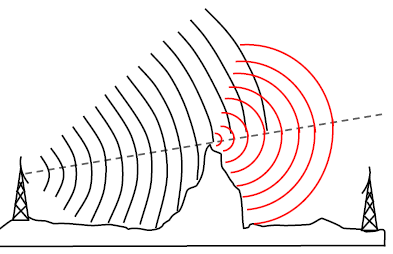
\includegraphics[width=0.85\linewidth]{images/diffraction} \end{center}

\begin{block}{Approche théorique}
\phantomsection\label{approche-thuxe9orique}
L'approche théorique repose sur des modèles mathématiques basés sur les
principes de la physique des ondes. Ces modèles prennent en compte les
phénomènes de diffraction, de réflexion et d'absorption. Parmi les
modèles théoriques les plus connus, on trouve :

Le modèle de réflexion sur le sol, prend en compte deux trajets : un en
ligne directe et un autre obtenu par réflexion sur le sol.

Les modèles de Walfisch-Bertoni et d'Ikegami, décrits dans
{[}Granatstein (2008){]}, intègrent les effets de diffraction des ondes
au niveau des toits d'immeubles. Ces modèles sont particulièrement
pertinents lorsque l'antenne est placée au-dessus des bâtiments et que
le récepteur se trouve en contrebas, dans une rue.
\end{block}
\end{frame}

\begin{frame}{Approche empirique}
\phantomsection\label{approche-empirique}
L'approche empirique peut être illustrée par le modèle de
\textbf{Delisle-Egli}, présenté dans \cite{Granatstein2008}, qui est un
modèle de propagation en milieu urbain.

Il se base sur un grand nombre de mesures effectuées dans des villes des
États-Unis,\\
qui ont permis d'établir la formule suivante pour l'atténuation de la
puissance d'un signal :
\end{frame}

\end{document}
